
\documentclass[nocopyrightspace, 10pt]{sigplanconf}

% The following \documentclass options may be useful:
%
% 10pt          To set in 10-point type instead of 9-point.
% 11pt          To set in 11-point type instead of 9-point.
% authoryear    To obtain author/year citation style instead of numeric.

\usepackage{natbib}
\usepackage{url}
\usepackage[squaren,thinqspace,binary]{SIunits}

\usepackage{hyperref}
\newcommand\fnurl[2]{%
  \href{#2}{#1}\footnote{\url{#2}}%
}

\let\fourth\relax               % Undefine a macro
\let\second\relax               % Undefine a macro
\let\degree\relax               % Undefine a macro
\let\cdot\relax                 % Undefine a macro
\usepackage{array}
\usepackage{amsmath}
\usepackage{amssymb}
%\usepackage{mathabx}
\usepackage{mathtools}
\usepackage{multirow}
\usepackage{bussproofs}
\usepackage{verbatim}
\usepackage{fancyvrb}
\usepackage{float}
\usepackage{graphicx}
\usepackage{subcaption,placeins}
\usepackage{setspace}
%\usepackage[tight,footnotesize]{subfigure}
% \usepackage{subfigure}
\usepackage{caption}

\usepackage[]{algorithm2e}
\usepackage{listings}
\usepackage{xcolor}

\usepackage{tabu}

% Display notes/comments with todonotes:
\usepackage[disable]{todonotes} % notes/comments not showed
% \usepackage[draft]{todonotes} % notes/comments showed

\newcommand{\fix}[1]{\texttt{\small #1}}
\lstset{
    inputencoding=utf8,
%    backgroundcolor=\color{white},
    tabsize=4,
    rulecolor=,
    upquote=true,
%    aboveskip={1.5\baselineskip},
    columns=fixed,
    showstringspaces=false,
    extendedchars=true,
    breaklines=true,
    prebreak = \raisebox{0ex}[0ex][0ex]{\ensuremath{\hookleftarrow}},
    frame=single,
    showtabs=false,
    showspaces=false,
    showstringspaces=false,
    basicstyle=\scriptsize\ttfamily,
    identifierstyle=\ttfamily,
    keywordstyle=\ttfamily\color[rgb]{0,0,1},
    commentstyle=\ttfamily\color[rgb]{0.133,0.545,0.133},
    stringstyle=\ttfamily\color[rgb]{0.627,0.126,0.941},
}



%\makeatletter
\lstdefinelanguage{llvm}{
  morecomment = [l]{;},
  morestring=[b]", 
  sensitive = true,
  classoffset=0,
  morekeywords={
    define, declare, global, constant,
    internal, external, private,
    linkonce, linkonce_odr, weak, weak_odr, appending,
    common, extern_weak,
    thread_local, dllimport, dllexport,
    hidden, protected, default,
    except, deplibs,
    volatile, fastcc, coldcc, cc, ccc,
    x86_stdcallcc, x86_fastcallcc,
    ptx_kernel, ptx_device,
    signext, zeroext, inreg, sret, nounwind, noreturn,
    nocapture, byval, nest, readnone, readonly, noalias, uwtable,
    inlinehint, noinline, alwaysinline, optsize, ssp, sspreq,
    noredzone, noimplicitfloat, naked, alignstack,
    module, asm, align, tail, to,
    addrspace, section, alias, sideeffect, c, gc,
    target, datalayout, triple,
    blockaddress, metadata
  },
  classoffset=1, keywordstyle=\color{purple},
  morekeywords={
    add, fadd, sub, fsub, mul, fmul,
    sdiv, udiv, fdiv, srem, urem, frem,
    and, or, xor,
    icmp, fcmp,
    eq, ne, ugt, uge, ult, ule, sgt, sge, slt, sle,
    oeq, ogt, oge, olt, ole, one, ord, ueq, ugt, uge,
    ult, ule, une, uno,
    nuw, nsw, exact, inbounds,
    phi, call, select, shl, lshr, ashr, va_arg,
    trunc, zext, sext,
    fptrunc, fpext, fptoui, fptosi, uitofp, sitofp,
    ptrtoint, inttoptr, bitcast,
    ret, br, indirectbr, switch, invoke, unwind, unreachable,
    malloc, alloca, free, load, store, getelementptr,
    extractelement, insertelement, shufflevector,
    extractvalue, insertvalue,
  },
  alsoletter=\%,
  keywordsprefix=\%,
}

%------------------------------------------------------------------------------
%\doublespacing
\begin{document}


\title{Scaling Computer Go Using OpenMP and MPI}
\subtitle{CS 484 - Parallel Programming Final Project}


\authorinfo{Waren Kemmerer \and Abdul Dakkak \and\\ Xun Jian \and Palash Sashittal}
           {}
           % {University of Illinois at Urbana-Champaign}
           {\{kemmere2, dakkak, xunjian1, sashitt2\}@illinois.edu}

\conferenceinfo{CONF 'yy}{Month d--d, 20yy, City, ST, Country} 
\copyrightyear{20yy} 
\copyrightdata{978-1-nnnn-nnnn-n/yy/mm} 
\doi{nnnnnnn.nnnnnnn}

\maketitle

\begin{abstract}

There has been extensive research on the strategy and tactics involved in Go (the game) by both professional players and computer scientists. In this report we present a parallelized implementation of a Monte-Carlo algorithm for computer Go by modifying  Pachi~\cite{pachi} -- a state-of-the-art Go AI engine. Scaling is achieved though the utilization of both OpenMP (to scale across cores) and MPI (to scale across nodes) and incorporating these modification into the original Monte Carlo source code and game engine of Pachi\footnote{The source code for this project along with the data presented is found at \texttt{https://github.com/abduld/cs484}}. We present the performance of our parallel implementation relative to the base performance of the original Monte Carlo implementation in Pachi. We then evaluate our algorithm as a function of the number of MPI ranks and OpenMP threads. Evaluation are obtained for both $9 \times 9$ and $19 \times 19$ boards and demonstrate both the effectiveness and scalability of our algorithm.  


\end{abstract}

\section{Introduction}

Go is an ancient Asian board game that has simple rules but produces extremely complex game play due to game size and possible move combinations.  The board game of Go has proved to be an exciting challenge in the field of Artificial Intelligence. Due to its inherent solution complexity (relative to chess), the game had been deemed impossible for computers to tackle as recent as 2005~\cite{gohard}.  However, with the advent of new AI techniques, Go has since become popular among researchers. As many of the techniques used to solve Go map directly into many other algorithms such as A*, beating a top Go player remains an important goal within AI research. Recognizing its importance the \textit{Ing Prize} was setup from $1993-2000$, which promised a reward of $\$1.4$ million dollars for first computer to beat a profession. Despite many attempts it was never claimed during that time.

There are strict time constraints in the game Go that add an additional degree of challenge to computational solutions. The game length is fixed at 60 minutes per player. Thus, since speed of the algorithm is critical, a computer must make decisions quickly, and thus the time alloted to explore games is limited. As a result, exploring multiple game moves in parallel can be very advantageous.

Due to the size of the game space, a complete playout of all possible games is not computationally feasible. Additionally, without an evaluation function, traditional game tree search techniques have been shown to be ineffective. Nevertheless, recent advances have shown that algorithms that do not fully explore the game-space or rely on an evaluation function, such as Monte-Carlo and Monte-Carlo Tree Search (MCTS) work well for Go. 

This report is organized as follows: We first describe the game Go as well as some of the rules. We then detail why Go is a difficult problem by relating it to chess and comparing their computational complexity. We then discuss the Monte Carlo algorithm and the modifications made within the Pachi framework to enable  OpenMP and MPI utilization. The results are then shown in the following section. After discussing our results, we conclude with future work.


\begin{figure}
\begin{center}
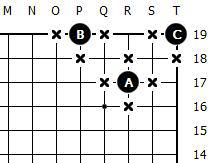
\includegraphics[width=0.3\textwidth]{liberties.jpg}
\end{center}
\caption{Example showing liberties for stones on the board. The liberties of \textbf{A}, \textbf{B} and \textbf{C} are marked with crosses.}
\label{liberties}
\end{figure}

\section{What is Go ?}

Go is a zero-sum board game involving two players. It's roots trace to at least in the 6th century B.C. in what is modern-day China. As one of the oldest board game in existence, it was considered one of the four essential arts of a cultured Chinese scholar in antiquity. The number of possible games is vast ($10^{761}$ compared to only $10^{120}$ possibilities in chess), despite having simple rules. Strategy and tactics involved in mastering the game require years of study and there are dedicated schools for the game.


\subsection{Rules}
Go is played on a square grid of a given size. $19 \times 19$ is the most popular, but smaller boards such as $13 \times 13$ and $9 \times 9$ are also used for beginners or for short games. Two players choose a white or black color and alternate place stones on the vacant intersections of the grid lines. Black makes the first move and white is awarded $6.5$ points because of this disadvantage.


Once stones are placed on the board they cannot be moved. Adjacent stones of the same color form a connected group, and the objective of the game is to have the largest connected group. A group shares liberties, which are vacant points adjacent to a group. When a group runs out of all liberties, then it is captured and the stones are physically removed from the board. For example, in Figure~\ref{liberties}, the liberties for stones \textbf{A}, \textbf{B} and \textbf{C} are marked with crosses.

A basics of Go is that stones must have at least one liberty to remain on the board. An enclosed liberty is called an eye and if a group has two separate eyes then it is said to be completely alive. Such a group cannot be captured even if surrounded.

Figure~\ref{capture} shows two configuration. In case \textbf{A}, we have a group of black stones which are not in immediate danger of being captured. A white move at \textbf{A} is not allowed, since it would be surrounded and would be suicide. If white however was to play at \textbf{B}, it would capture all the black stones surrounding \textbf{B}, since no liberties are left for black. the white player would then remove all the black pieces that have been captured.


\begin{figure} 
\begin{center}
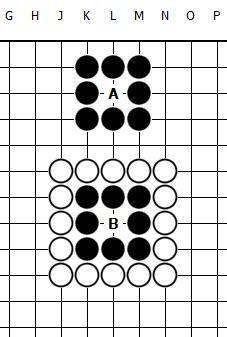
\includegraphics[scale=0.45]{capture.jpg}
\end{center}
\caption{Example showing how to capture a group. White can capture the black stones by placing a stone at \textbf{B}, but white cannot insert a stone at \textbf{A} since it would be suicide.}
\label{capture}
\end{figure}


The other rule in Go is the \textit{ko} rule. It states that the a play must not repeat the same configuration of an immediate previous move. Such moves are not allowed and thus a player must either pass or play at another position in the board. Without the \textit{ko} rule a game can be infinite.

\begin{figure}
\begin{center}
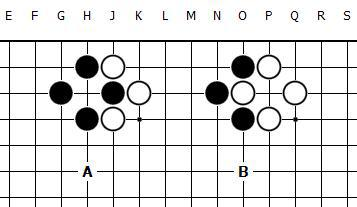
\includegraphics[width=0.45\textwidth]{ko.jpg}
\end{center}
\caption{Example showing the \textit{ko} rule. Capturing the black stone in \textbf{A} would result in the configuration in \textbf{B}. Similarly, capturing the white stone in \textbf{B} results the \textbf{A} configuration. The \textit{ko} rule disallows repeating the immediate previous state.}
\label{ko}
\end{figure}


An extension to \textit{ko} rule is the \textit{superko} rule. This rule states that a play is illegal if it would have the effect (after all steps of the play have been completed) of creating a position that has occurred previously in the game. However, it doesn't bar a player from passing. This ensures that the game eventually moves to an end by preventing indefinite repetition of the same positions.


The objective of the game is to have surrounded a larger total area of the board with one's stone than the opponent by the end of the game. The number of points occupied or completely surrounded by stones of a player (and \textit{komi} which are some points given to white player as a compensation for playing second) is the score, and the player with higher score wins the game. The game ends when both players consecutively play a pass move, when one of the players resigns, or when there are no more remaining legal moves on the board. Thus unlike with Chess, where the objective is to kill the opponent, the strategy in Go is to have the biggest sphere of influence.

Although there are minor differences between rule sets used in different countries, these differences do not change the tactics of the game. For example, some rule sets allow suicide moves while some do not. A suicide move is when a player places a stone such that it has no liberties on the board. This kind of play will only be useful in a limited number of circumstances.

\section{Differences from Chess}

It is worth describing why Go is a harder problem than Chess and discuss some of its computational complexity. While it is well publicized that Deep Blue (developed by IBM) was able to beat the chess grandmaster Garry Kasparov under chess time rules in 1997~\cite{deepblue}, computer Go has yet to defeat a professional using traditional rules. The complexity of Go is due to four factors:

\begin{enumerate}
\item \textbf{Evaluation Function}: The performance of computer chess in the 90s was mainly due to the $\alpha \beta$-pruning algorithm, which when applied with \textit{minmax} exploration prunes trees, do no explore losing paths. The $\alpha \beta$-pruning algorithm requires an evaluation function (the ability to be able to immediately determine whether a move is good or not) given a board state. While such an evaluation function exists in Chess, it does not exist in Go~\cite{abvs}. In Go, one has to play out the entire the game, reach the end, and then determine from the final board state whether the game is won or lost.
\item \textbf{Board Size}: The size of the board in Go is 19x19 (or 9x9 depending on the rules) while in chess it is 8x8 in chess. The state of exploration is therefore larger in Go. There are $3^{361}$ legal moves in Go, and without pruning the exploration tree is $361!$~\cite{mathgo}. Furthermore, the board is initially empty in Go unlike in chess. This means that the entire board can be explored in Go initially whereas in chess only half of the board can be explored (since half of the chess board is initially occupied by game pieces). 
%Finally, whereas in chess one has a fixed rule of how the pieces can be moved, no such rules exists in Go. 
\item \textbf{Branching Factor}: The branching factor of the exploration tree corresponds to the valid moves one can make during each turn. In Go around $250$ positions are valid at each turn while it is $35$ in chess~\cite{branch}. 
\item \textbf{Pass Rule}: In Go a player is allowed to pass. Therefore when performing the game simulation one needs to simulate the passing behavior of an opponent.
\end{enumerate}

When combining all of the above the search state space of Go is EXPTIME~\cite{exptime,exptime2}.

\section{Monte Carlo in Go}
Monte Carlo methods invoke the law of large numbers by performing many randomized simulations and selecting the most probable solution gained from the largest percentage of the performed simulations. We use randomized simulations to evaluate Go positions and build a game vector called a \textit{playout}. 

Each random move is evaluated by a number of \textit{playouts}. In each playout, the games are played-out to the very end by selecting moves at random. The move that gets the maximum number of wins at the end of the playouts is chosen.

\subsection{Exploration vs Exploitation}

A simple Monte Carlo algorithm gives more importance to exploration than exploitation. Exploration is trying out larger section of the sample space while exploitation is focusing on simulations of the best candidate moves. Thus, while exploration involves playing out more moves at a particular state on the board, exploitation involves trying out different playouts for the same move to make sure that the win/loss ratio assigned to that move is correct. 

This flaw is nullified by running several Monte Carlo engines in parallel. This ensures that each moves receives a sufficient number of playouts and will be discussed in greater detail in next section.

\section{Parallel Monte Carlo}

We parallelize Pachi Go in two stages (OpenMP and MPI).  Both OpenMP and MPI function independently from one another and can be considered separately or together depending on the desired execution.  Several modifications to the original Monte-Carlo code and Pachi game engine were necessary in order to accomplish parallelization on the OpenMP and MPI levels.  We describe these modifications in the sections below.

\subsection{Code Modifications for OpenMP}

\subsubsection{Move Generation}

In order to determine the next move, the original Monte Carlo engine places a stone randomly on the board and then plays a random game to completion, determining a possible outcome following the first move.  After recording the results, the initial board (from the start of the turn) is again considered and a new potential location is chosen and its subsequent playout occurs.  This process continues until playout time has expired.  The algorithm collectively adds together the number of games and wins associated with each location on which a stone can be placed.  %Additional variables and algorithms are used to ensure that the moves considered legally conform to the rules of the game.  
By finding the ratio of games won to games lost for each location, the position with the highest win ratio is chosen as the next move.   If moves corresponding to a possible win are found, the program passes.

%In order to provide thread level parallelism to the algorithm, we first consider thread division using OpenMP. 
To perform OpenMP parallelization, we need to divide the exploration task among the different threads. One way to evenly divide the tasks is to evenly divide all the available next moves evenly between threads; however, this require maintaining an active list of available next moves, which is a feature not currently in the original algorithm.  Instead we recognize that letting the different threads randomly explore possible next moves on their own should also allow relatively balanced exploration across all possible next moves. We let the threads update a shared win/loss array, which holds the current win/loss array corresponding to each explored next move, to collectively improve the accuracy of the win/loss ratios of the explored moves. A key element of this division is to ensure that the random variable used to generate moves and determine playout outcomes are truly thread independent.  Without such independence, certain board positions might be inaccurately over- or under-represented in the total number of first moves.  Additionally, the independence of random number spaces is necessary to ensure that game playouts are not correlated between threads, which leads to the undesired scenario where some possible moves are under explored compared to others.




\subsubsection{Game Randomization}

%Conceptually, the outcome of each  game playout should be influence only by the state of the board at the beginning of the turn, the uniquely random first move chosen, and the uniquely randomized sequence of playouts.  
The original Monte Carlo algorithm takes advantage of the small board size relive to the typical random number space to utilize a fast random number generator because speed is of the essence.  In order to ensure that each thread is independent, we therefore need to seed this fast random number generator using unique numbers for each thread.  Additionally, to ensure that repeated games do not result in identical outcomes, we must ensure that the numbers used to seed the random number are also uniquely random.  

In order to accomplish this, we use the computer's time in 
 microsecond to seed the \texttt{srand} function at the beginning of the game.  This ensures uniquely random outcomes between games.  We then use iterative values of \texttt{rand} to seed a thread independent value to the \texttt{fast\_random} function at the beginning of each \texttt{genmove}.  As \texttt{rand} is significantly slower than the fast random function, this is only performed only once per move command.  We then use a modified thread independent \texttt{fast\_rand} function to provide randomness within the thousands of games explored, each with their thousands of possible moves.  This ensures that each move and each playout are uniquely random between threads.

Failing to account for the above modifications results in race conditions between each thread and the random number generator, which due to the original \texttt{fast\_rand} design could possibly result in the evaluation of highly correlated games.

\subsubsection{Flow Control \& Variable Protection}

	Additional modifications were made to the flow control elements provided in the code.  Unfortunately, the original Monte Carlo source code has complicated control flow and is riddled with go-to and continue statements.  In order adhere to OpenMP standards, \texttt{goto} statements were eliminated from the parallel version of the code --- since the originial control flow graph was irreducible.  This was accomplished using loop transformations, privatization, and locks.
	
The remaining alterations to the Monte Carlo algorithm are primarily used to ensure that variables associated with each move and playout are correctly protected.  Read-only values are freely shared between threads, unique and independent variables are privatized, and cumulative variables are protected through a series of locks and reductions.  

After parallel exploration is complete, the cumulative results are compared and the best result is chosen as the next move.  Relative to the parallel exploration, this comparison is trivial and is therefore not considered for parallelization.
	
\subsection{Code Modifications for MPI}
\subsubsection{MPI Compatible Environment}


\begin{algorithm}
    \ForEach{MPI Rank}{
         \eIf{MPI Rank = 0}{
            \While{input is valid}{
                $read$ input stream into local buffer\;
                $broadcast$ input stream to all ranks\;
                $parse$ IO and created new commands using socket interface\;
            }
          }{
            \While{input is valid}{
                $read$ input stream into local buffer\;
                $parse$ IO and execute silently\;
            }
          }
    }
 \caption{Pseudo-code of the Pachi engine to handle execution across MPI ranks.}
 \label{alg:monte-carlo_mpi_mod_pseudocod}
\end{algorithm}



Supporting the framework for MPI parallelism proved to be far more challenging than expected.  Given the engine-driven nature of the code, individual ranks each needed to instantiate a unique engine which could then provide additional game-space exploration.  The essence of the modifications is shown in Algorithm~\ref{alg:monte-carlo_mpi_mod_pseudocod}.

In order to accomplish this, engine generation and handling needed to be MPI rank aware.  In the native code, an engine receives instructions from the player using textually based commands received from the \texttt{stdio} stream and stored in a temporary buffer.  These commands are then parsed by the engine which, executes the corresponding commands based on the instructions received.  Throughout the process, the Pachi engine communicates with the player engine through a series of \texttt{gtp} sockets in order to properly ensure that the player engine is aware of the current game state.

We first note that only one engine can access the \texttt{stdio} buffers and \texttt{gtp} sockets at a time.  If multiple engines attempt to read the input stream, two situations can occur.  In one case, only one engine receives the entire stream and subsequent engines receive nothing (which is unlikely).  In the second case, each engine will only receive a subset of the stream, resulting in corrupted and unusable messages.  With concern to the multiple accesses to \texttt{gtp} socket accesses, if multiple states or confirmation messages are received by the player, the player will crash or assume that the engine has resigned. 


\begin{algorithm}
    Generate seeds for each OpenMP thread\;
    \ForEach{OpenMP Thread}{
        $copy$ board's original state\;
        $make$ a random move\;
        $playout$ the game until the end\;
        $score$ the game to determine the winner\;
        $store$ the results collectively\;
        \eIf{MPI Rank = 0}{
            $recieve$ array from all ranks via a reduction collective\;
            $calculate$ the best move\;
            $broadcast$ the best move\;
          }{
            $send$ results to root\;
            $recieve$ the best move\;
          }
    }
 \caption{Pseudo-code of the Monte Carlo function to handle execution across OpenMP threads and MPI ranks.}
 \label{alg:monte-carlo_omp_mod_pseudocod}
\end{algorithm}

In order to ensure that only one MPI rank accesses the input stream and output sockets, we dedicate MPI rank 0 as the only engine that can access with either interface.  MPI rank 0 reads the input stream and broadcasts its copy of the internal buffer to all other ranks.  Each rank then independently parses and executes all commands in the buffer.  In order to ensure that rank 0 is the only engine to perform socket communication, separate executions are created for ranks greater than 0 in which all socket communication has been removed.  The pseudo-code for the modifications required to handle the MPI/OpenMP hybrid is shown in Algorithm~\ref{alg:monte-carlo_omp_mod_pseudocod}.

\subsubsection{MPI Monte Carlo Implementation}

To further combine the results of all games across all MPI ranks, we perform an MPI reduction of the game statistics.  These specifically include the number of wins associated with each move and with the number of games explored along each move. The cumulative values are then analyzed by rank 0 which determines the best move and broadcasts the results.  Each MPI engine then executes the same move, which ensures consistency between the states of the different MPI engines.  

To achieve randomization between the MPI ranks, only a minor modification to our OpenMP scheme is necessary.  Instead of initially seeding our \texttt{srand} function using just the microsecond count of the computer, we now use the MPI rank in combination with the microsecond count to seed the \texttt{rand} function.  This ensure that all random numbers generated within the MPI ranks and within OpenMP threads of each MPI rank are unique.  This enables the independent exploration of the game space on both OpenMP and MPI levels.


\section{Evaluation}

We note that since the time interval associated with each move is programatically fixed, our code achieves no speedup relative to the original Monte Carlo algorithm.  Instead, the benefits of parallelization are manifested in the number of additional games that the program is able to explore.  These additional game simulations translate into more informed decision making by our program, which in theory should also be manifested in the outcome of the game.

We first consider the average number of game playouts associated with each level of parallelization relative to the original single threaded code.  Each level of parallelism (OpenMP thread level and MPI rank level) is considered independently from one another.  Results are further obtained for  MPI/OpenMP hybrid execution.  Due to simulation time constraints, we have chosen to demonstrate the effectiveness of our parallel code primarily using a $9 \times 9$ board for extensive testing.  Partial results have also been obtained using the full $19 \times 19$ board which further demonstrate the effectiveness of our algorithm.


\subsection{OpenMP Evaluation Using a $9 \times 9$ Board}


%\begin{figure*}
%  \centering
%  \begin{subfigure}[b]{\textwidth}
%    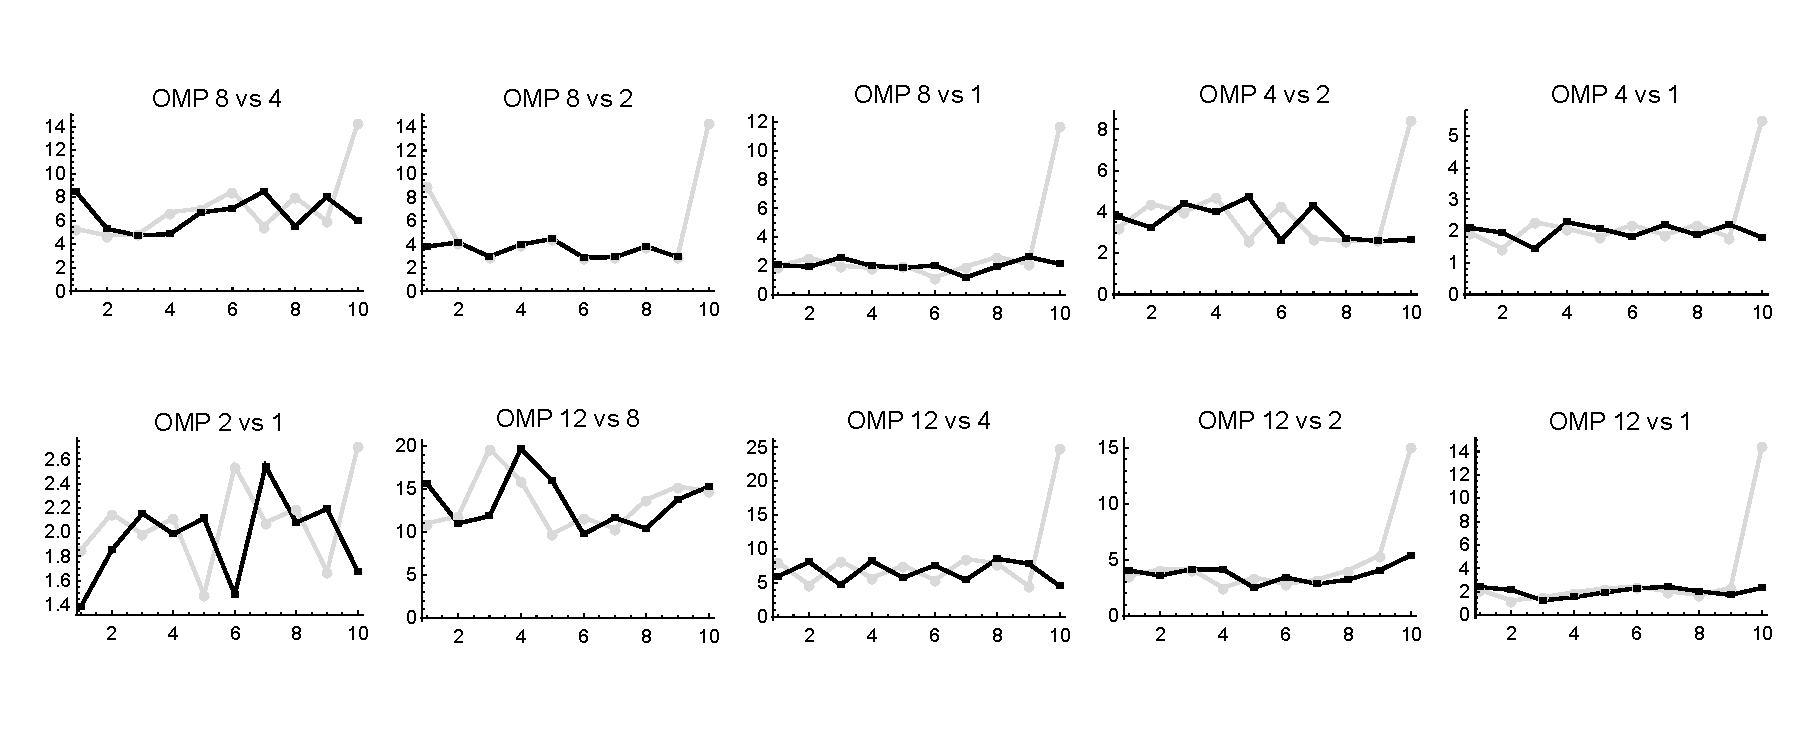
\includegraphics[width=\textwidth]{stev_1sec_OMP_vs.pdf}
%    \caption{Number of playouts for OpenMP using a 1 second time limit.}
%    \label{fig:playoutomp_1sec}
%  \end{subfigure}
%  
%  
%  \begin{subfigure}[b]{\textwidth}
%    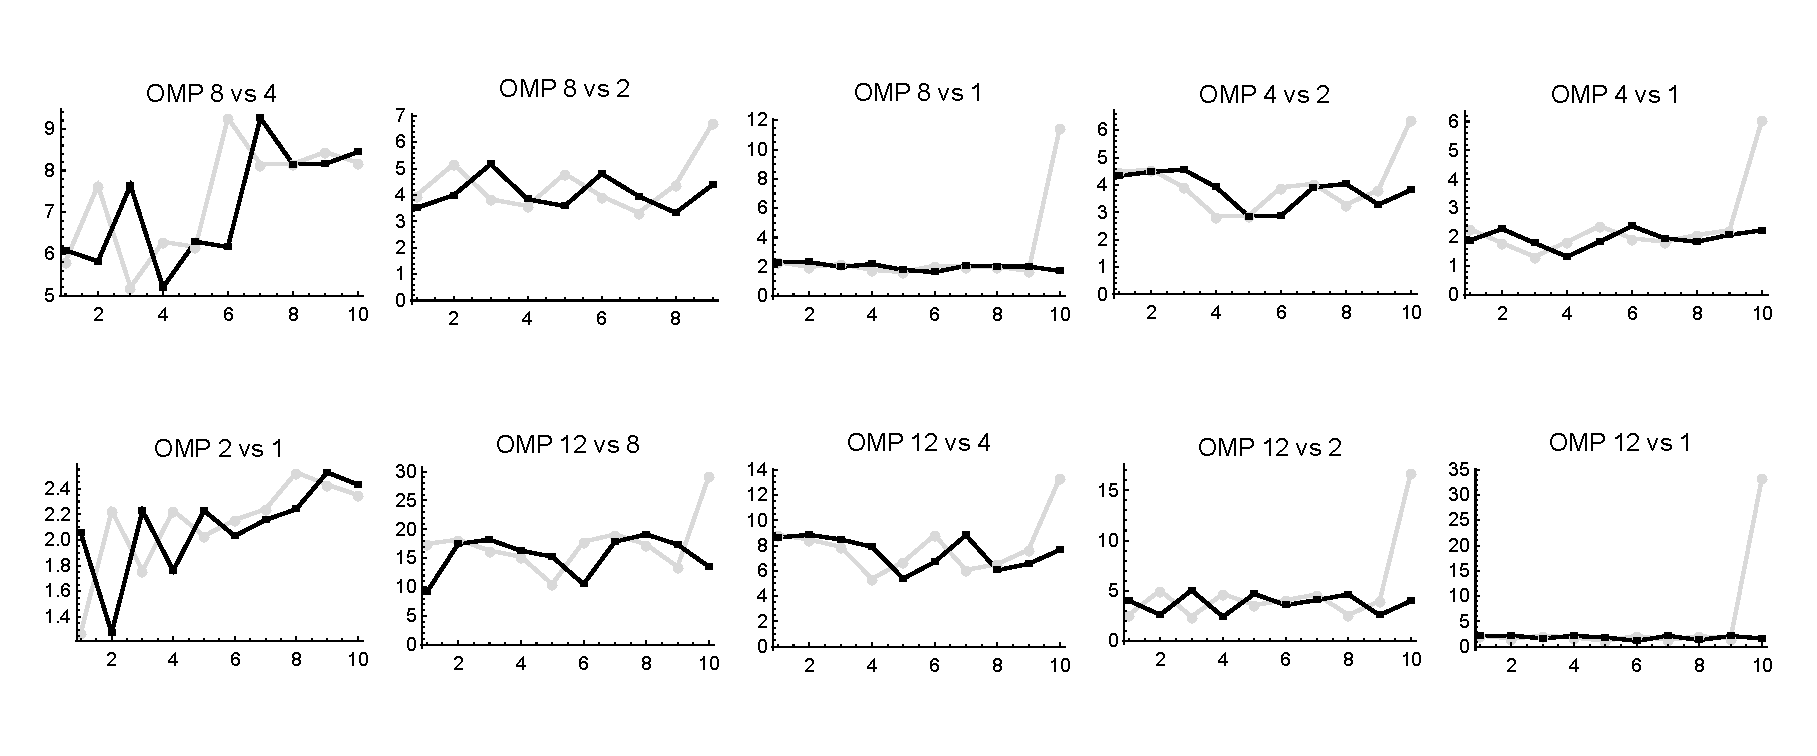
\includegraphics[width=\textwidth]{stev_60sec_OMP_vs.pdf}
%    \caption{Number of playouts for OpenMP using a 60 second time limit.}
%    \label{fig:playoutomp_60sec}
%  \end{subfigure}
%  \caption{Number of playouts for OpenMP using 1 and 60 second time limit. The $x$ axis shows how the number of playout vary across runs while the $y$ axis shows the millions of playouts performed. White which is our engine is shown in gray while the opponent is black.}
%  \label{fig:playoutomp}
%\end{figure*}

\begin{figure*}
\centering
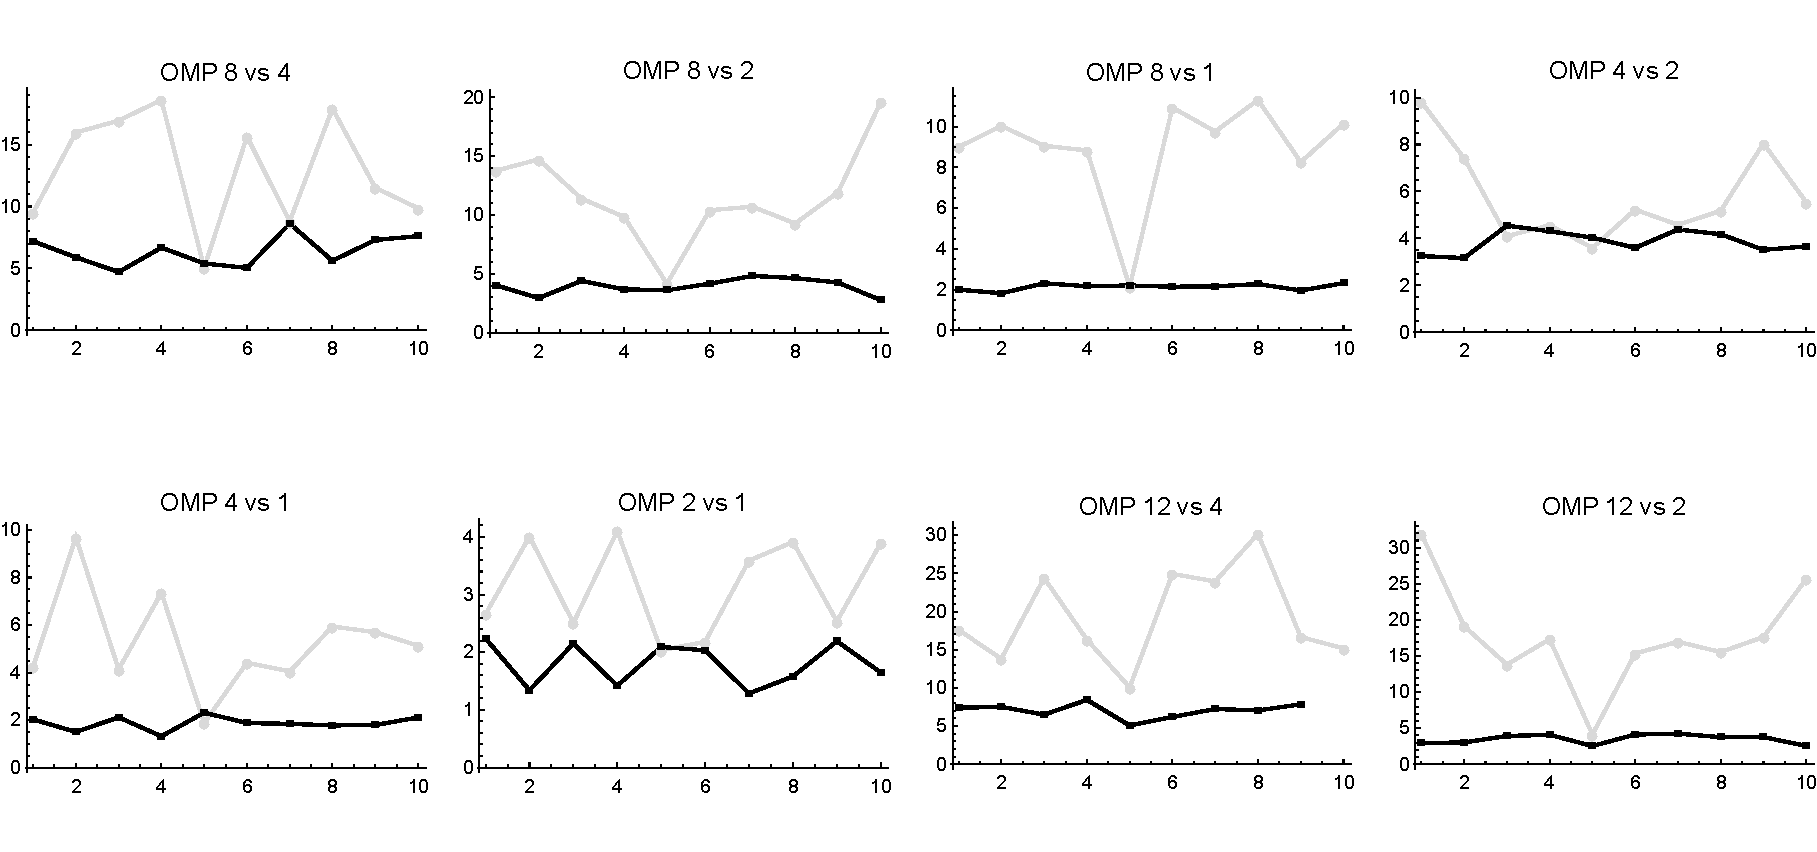
\includegraphics[width=\textwidth]{war_OMP_vs.pdf}
\caption{Number of playouts for OpenMP on a $9\times 9$ board using 1 second time limit. The $x$ axis shows how the number of playout vary across runs while the $y$ axis shows the millions of playouts performed. White (us) is compared against black which uses less OpenMP threads.}
\label{fig:playoutomp}
\end{figure*}


Figure~\ref{fig:playoutomp} shows the number of playouts performed as the number of OpenMP threads for white (us) and black (the opponent) varies. We observed that for every run the white player, which runs on more number of threads, performs more playouts, compared to the black player (running a smaller number of threads). We can also see that as we increase the number of threads, the rate at which the number of playouts increase at a constant rate. This shows that the code is scalable. 

%There are cases when the number of playouts performed by the white player is the same as the black player. This happens when the game terminates early or when the entire board has been explored. This is likely on a the small $9\times 9$ board, since the state space is small.

%AS can be seen the number of game simulations scales linearly with the number of threads. In some cases, where the game terminates early or when the opponent has around the same number of threads as us we see little difference. 

\subsection{MPI Evaluation Using a $9 \times 9$ Board}

%\begin{figure*}
%  \centering
%  \begin{subfigure}[b]{\textwidth}
%    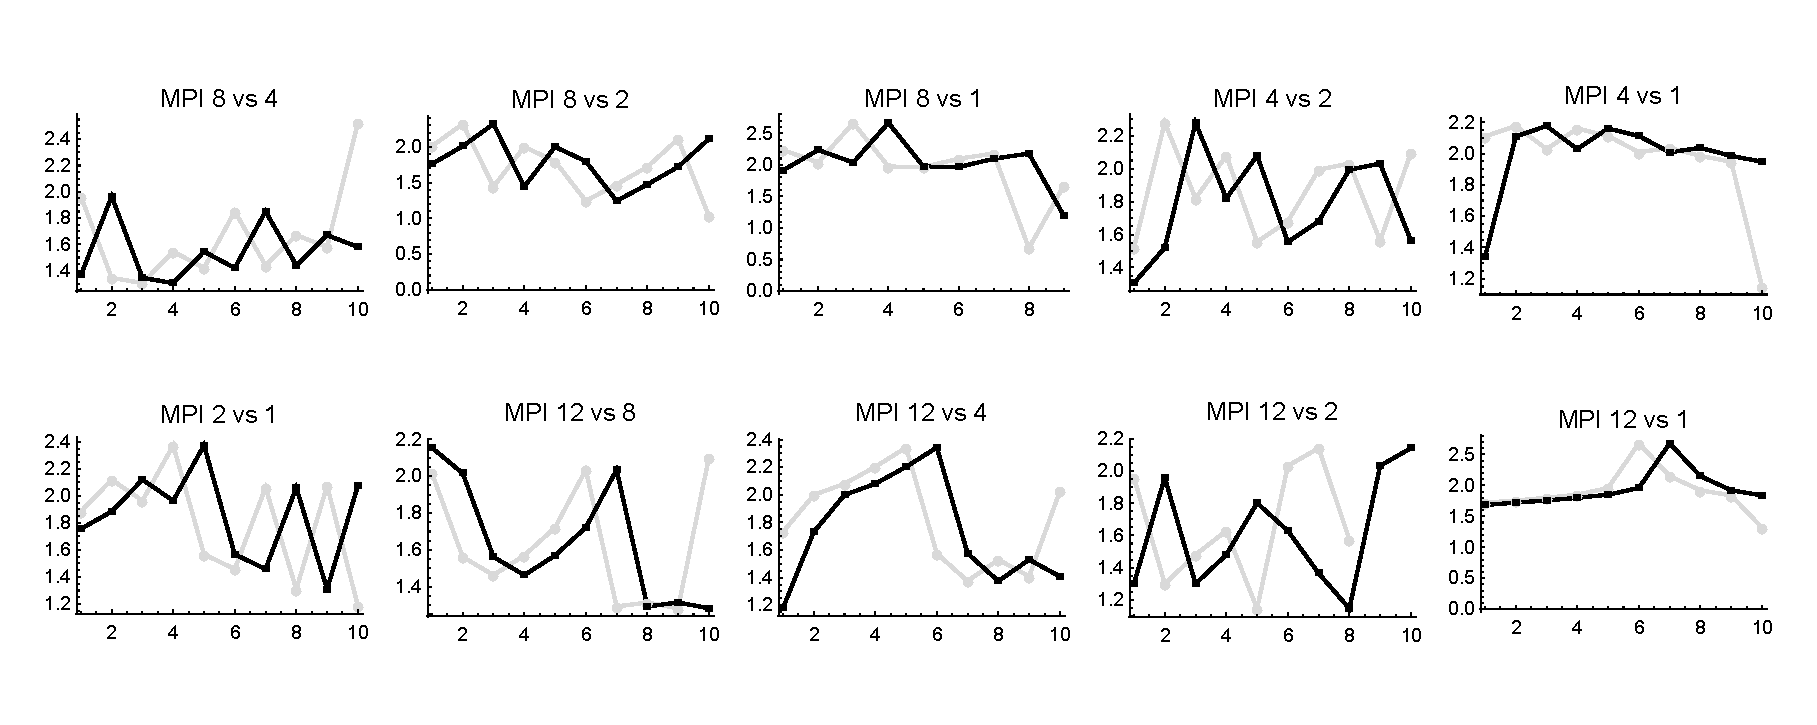
\includegraphics[width=\textwidth]{stev_1sec_MPI_vs.pdf}
%    \caption{Number of playouts for MPI using a 1 second time limit.}
%    \label{fig:playoutmpi_1sec}
%  \end{subfigure}
%  
%  
%  \begin{subfigure}[b]{\textwidth}
%    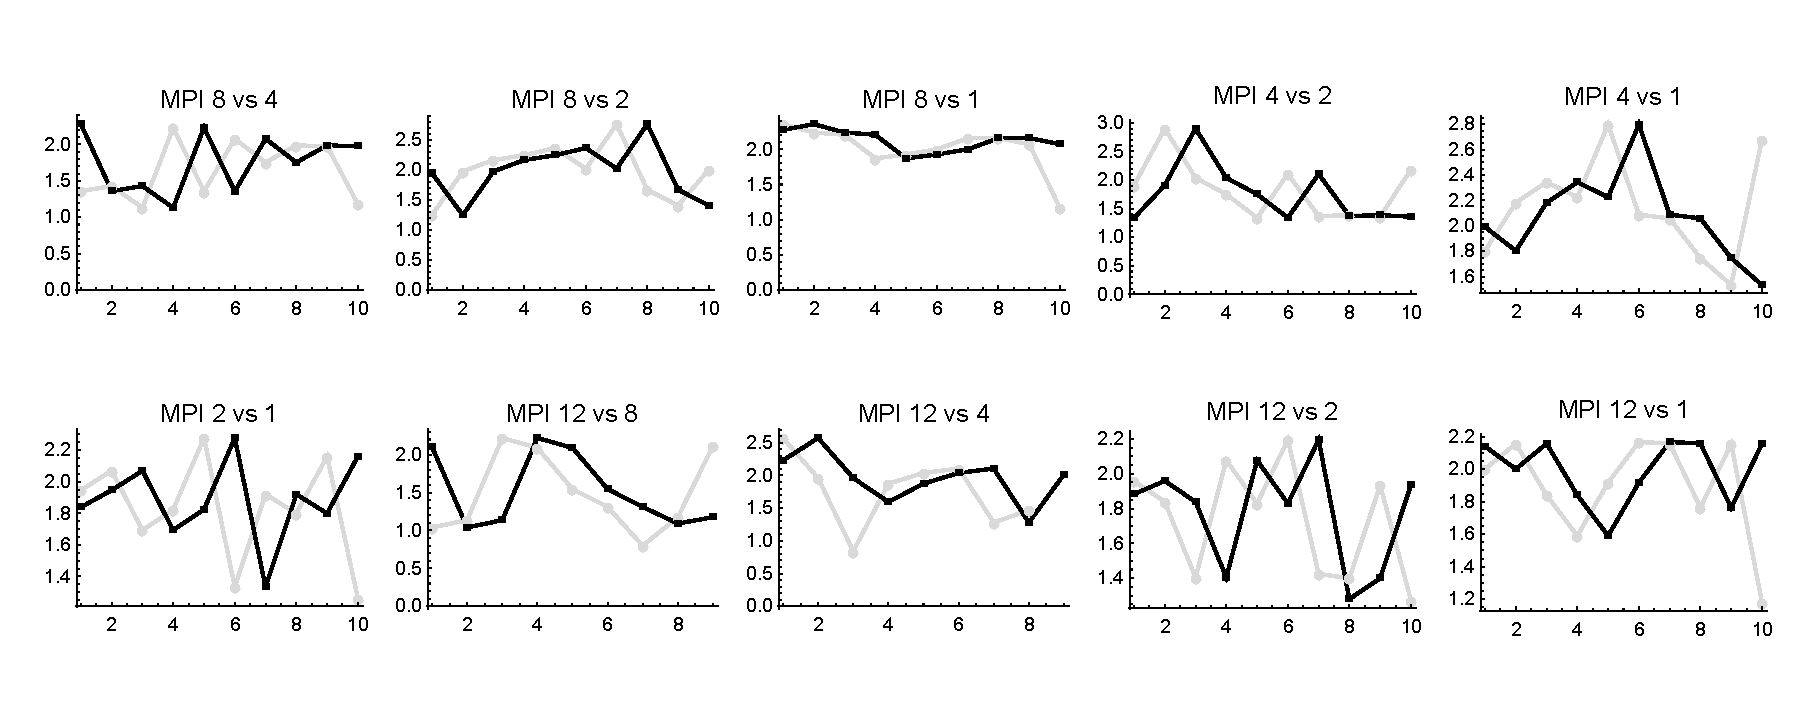
\includegraphics[width=\textwidth]{stev_60sec_MPI_vs.pdf}
%    \caption{Number of playouts for MPI using a 60 second time limit.}
%    \label{fig:playoutmpi_60sec}
%  \end{subfigure}
%  \caption{Number of playouts for MPI using 1 and 60 second time limit. The $x$ axis shows how the number of playout vary across runs while the $y$ axis shows the millions of playouts performed. White which is our engine is shown in gray while the opponent is black.}
%  \label{fig:playoutmpi}
%\end{figure*}

\begin{figure*}
\centering
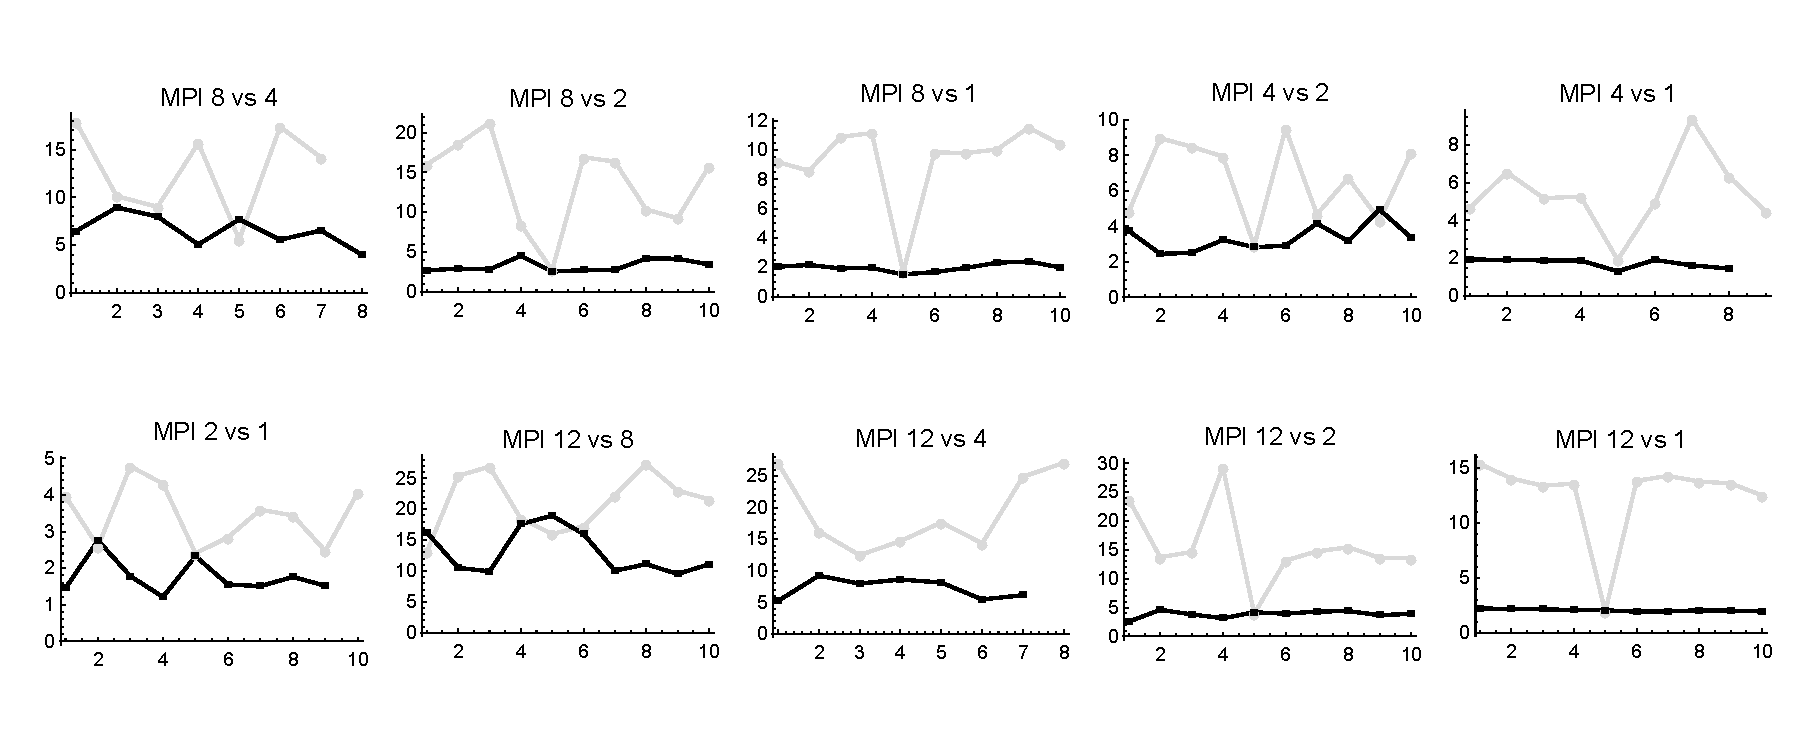
\includegraphics[width=\textwidth]{war_MPI_vs.pdf}
\caption{Number of playouts for MPI on a $9\times 9$ board using 1 second time limit. The $x$ axis shows how the number of playout vary across runs while the $y$ axis shows the millions of playouts performed. White (us) is compared against black which uses less MPI ranks.}
\label{fig:playoutmpi}
\end{figure*}

The number of playouts as we vary the number of MPI ranks is shown in figure~\ref{fig:playoutmpi}. The white and black lines show the performance of the white and black players respectively. The white player runs more ranks than the black player and has similar trend to the OpenMP case. The white player always outperforms the black player in terms of number of playouts. Since the size of the board is small, there is no noticeable improvement in performance of MPI processes as compared to OpenMP threads, but we do observe that there are measurable overhead in using MPI vs OpenMP.

\subsection{MPI/OpenMP Hybrid Evaluation Using a $9 \times 9$ Board}
The MPI/OPenMP hybrid executions vary both the number of MPI ranks and OpenMP threads. The results for hybrid executions obtained using TAUB are shown in figure~\ref{fig:playouthybrid}. We can see a significantly higher increase in the number of playouts performed as compared to both MPI or OpenMP cases. Thus, hybrid cases perform considerably better than MPI and OpenMP cases.

Figure ~\ref{fig:playouthybrid2} shows the number of playouts for different number of MPI Ranks and OpenMP threads relative to the original single threaded Monte-Carlo algorithm. The vertical bars on the left are for threads run on 2 MPI ranks and bars on the right are for 4 MPI ranks. It is clear that as number of OpenMP threads and MPI ranks are increased, there is an relatively consistent increase in the number of playouts performed. 

To further illustrate this consistency, the playout ratio normalized by the total number of threads in each run ($MPI rank \times OpenMP$ threads) is shown in Figure~\ref{fig:playouthybrid3}. Here we see that while the number of total threads increases, the increase in playout ratio is essentially a constant (see OpenMP 4, 8, and 12 for MPI rank 2). This directly shows the scalability of our algorithm.

%So a value of $1$ will indicate that the average number of playouts performed per thread is the same as the number of playouts performed when a single thread was run. It can be seen that for all cases the relative playouts per thread is less than $1$. This can be attributed to the locks and reductions performed by the code and to the fact that some portions of the code cannot be parallelized.

%For simplicity, in all cases, the single threaded execution is used as the baseline.  Data for all points is averaged over 10 games for each configuration.  Results are obtained using TAUB and are shown in Figure~\ref{fig:playouthybrid}. Due to execution timing constraints, results are reported only for the 9x9 board. 

\begin{figure*}
\centering
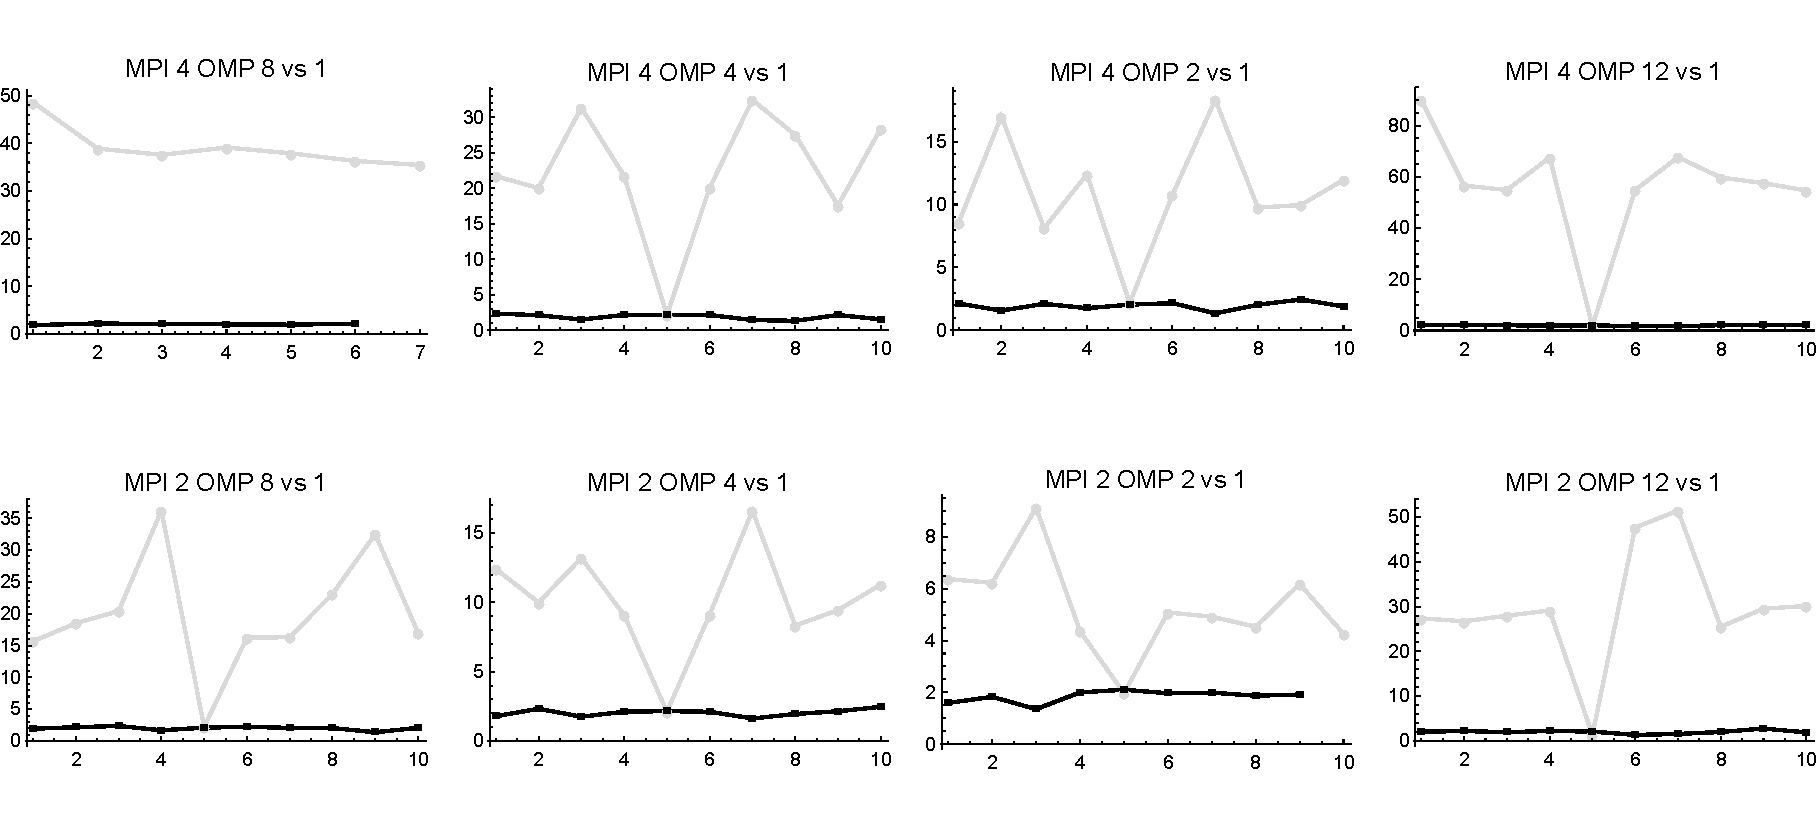
\includegraphics[width=\textwidth]{war_MPI_OMP_vs.pdf}
\caption{Number of playouts for MPI/OpenMP hybrid on a $9\times 9$ board using 1 second time limit. The $x$ axis shows how the number of playout vary across runs while the $y$ axis shows the millions of playouts performed. White (us) is compared against black which uses less MPI ranks or OpenMP threads.}
\label{fig:playouthybrid}
\end{figure*}

\begin{figure} 
\begin{center}
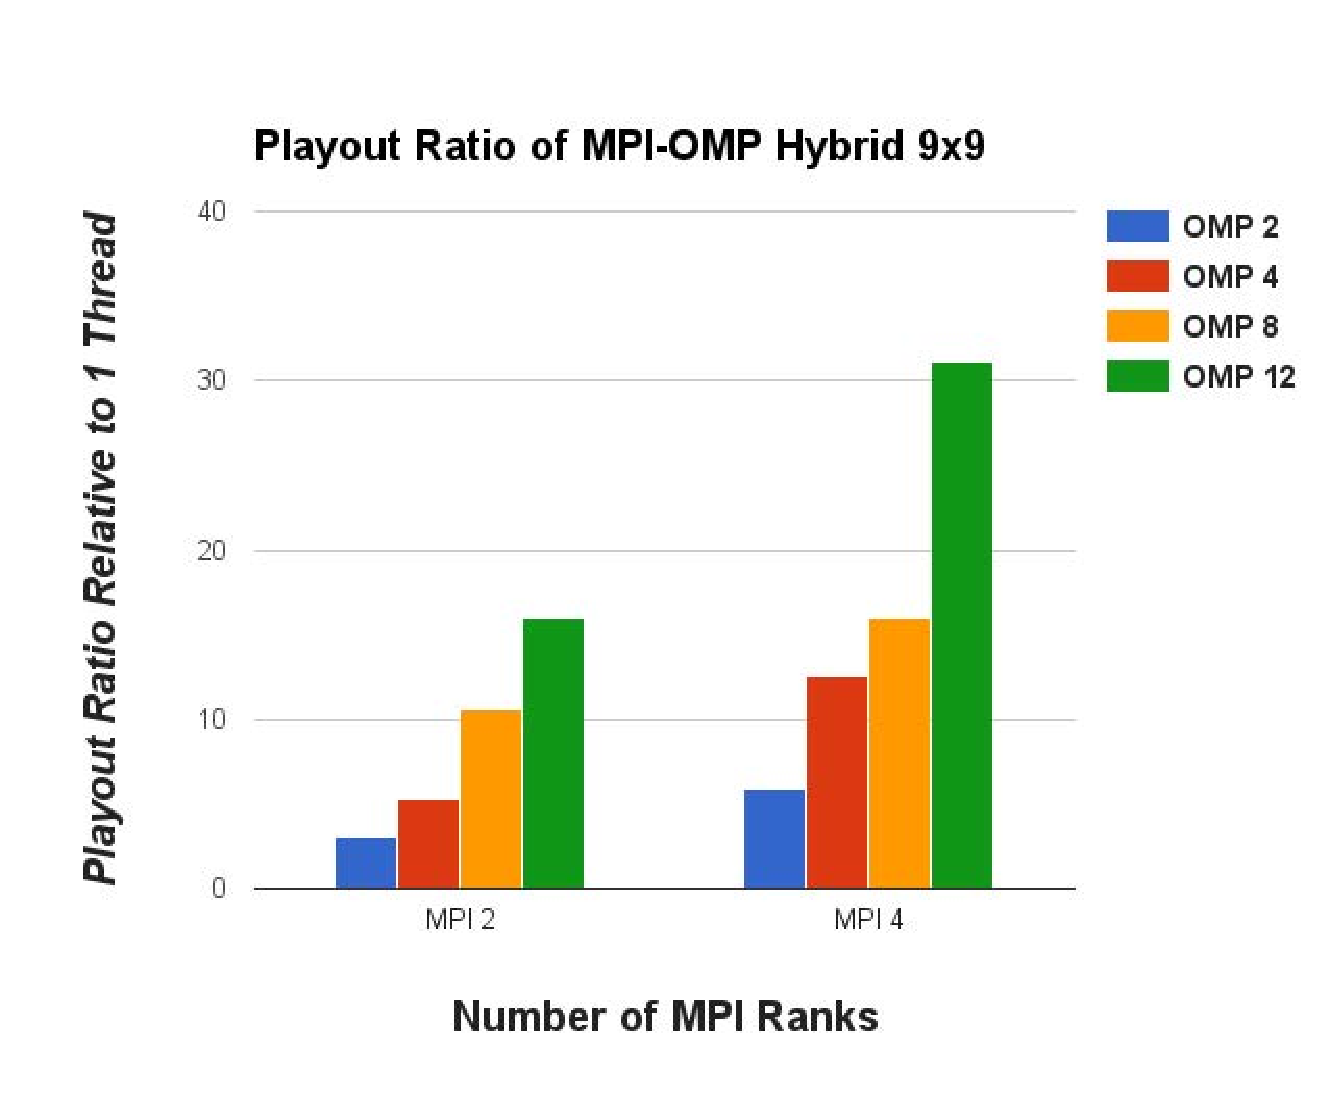
\includegraphics[width=0.45\textwidth]{MPI_OMP_hybrid_9x9_playout.pdf}
\end{center}
\caption{The ratio of games explored for competing MPI/OpenMP hybrid configurations on a $19 \times 19$ board averaged over all 10 games run on TAUB.}
\label{fig:playouthybrid2}
\end{figure}

\begin{figure} 
\begin{center}
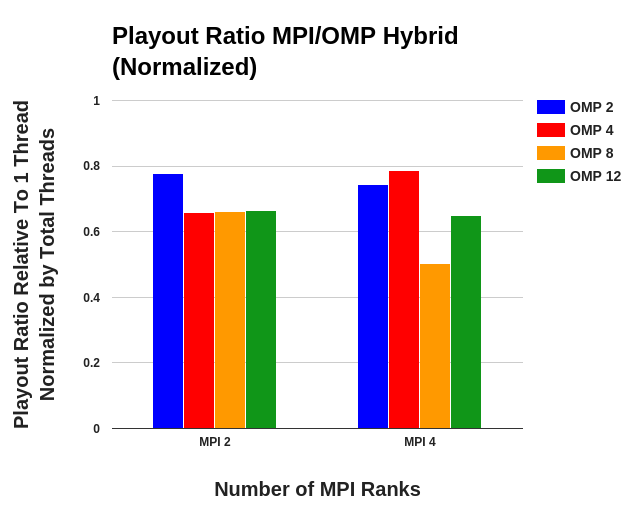
\includegraphics[width=0.45\textwidth]{playout_ratio_hybrid.png}
\end{center}
\caption{Normalized playout ratio for MPI/OpenMP hybrid on $9 \times 9$ boards run on TAUB. The normalization measures the thread factor advantage between competing MPI/OpenMP hybrid configurations.}
\label{fig:playouthybrid3}
\end{figure}

\subsection{OpenMP Evaluation Using a $19 \times 19$ Board}

Here we discuss the results generated from running simulations of games on $19\times 19$ boards in which we vary only the number of OpenMP threads associated with each player. The player associated with white varied the number of threads between 2, 4, 8 and 12 while the player associated with black varied the number of threads between 1 and 2.  In all OpenMP games played on the large board, the player with the larger number of threads was able to win 100\% of the time. The playout results of these experiments can be seen in Figure~\ref{fig:playoutompfull}.  In the graph we see that for a given baseline number of OpenMP threads, by increasing the number of OpenMP threads associated with the challenger (white) we increase the corresponding ratio between the number of playout games explored.  Conversely, we see that by for a given number of OpenMP threads associated with the challenger (white), by increasing the number of OpenMP threads associated with the baseline player (black), the resulting ratio decreases.  To demonstrate the consistency of these changes, we have normalized the playout ratios by dividing by the ratio of the number of OpenMP threads associated with each player.  The resulting plot can be seen in Figure~\ref{fig:playoutompfullnorm}.  In general, it can be seen that this ratio remains relatively constant, which clearly demonstrates that our OpenMP parallel implementation scalable for the levels of parallelism considered.

\begin{figure}
\begin{center}
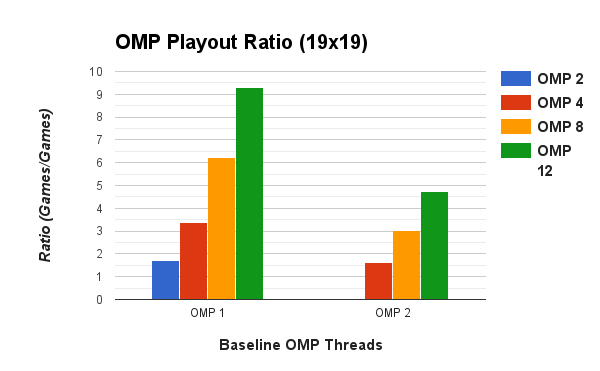
\includegraphics[width=0.45\textwidth]{omp_19_playout.png}
\end{center}
\caption{The ratio of games explored for competing OpenMP configurations on a $19 \times 19$ board averaged over all 10 games.}
\label{fig:playoutompfull}
\end{figure}


\begin{figure}
\begin{center}
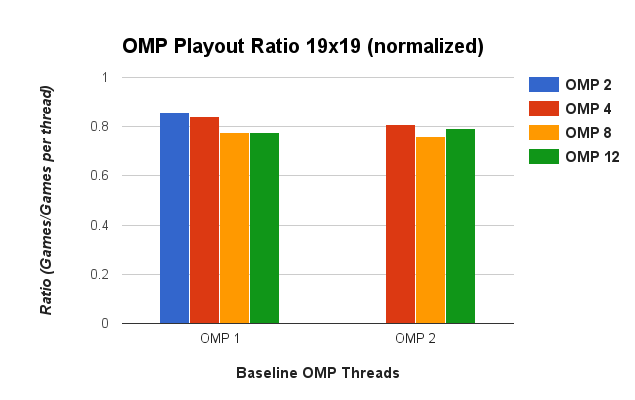
\includegraphics[width=0.45\textwidth]{omp_19_playout_norm.png}
\end{center}
\caption{Normalized playout ratio for OpenMP on $19 \times 19$ boards. The normalization measures the thread factor advantage between competing OpenMP configurations.}
\label{fig:playoutompfullnorm}
\end{figure}

\begin{figure*}
\centering
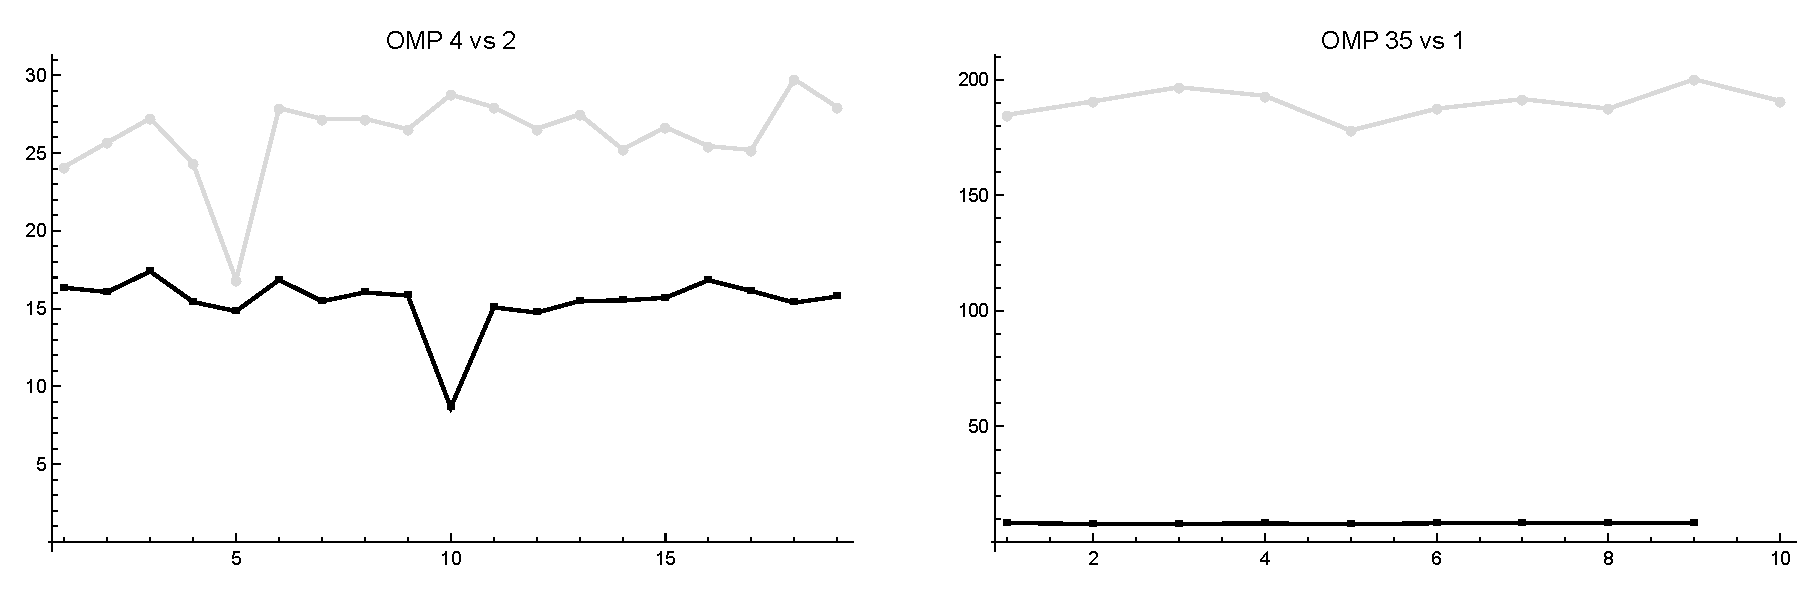
\includegraphics[width=\textwidth]{adk_19_vs.pdf}
\caption{Number of playouts for OpenMP on a $19\times 19$ board using 5 second time limit. The data was collected on a 36 core machine. The $x$ axis shows how the number of playout vary across runs while the $y$ axis shows the millions of playouts performed. White (us) is compared against black which uses less OpenMP threads ranks.}
\label{fig:playoutomp5limit}
\end{figure*}

If we consider a full game played on a 36 core Amazon AWS instance, we notice significant improvements. The space was not fully explored, since it takes over an hour to play a game to completion, but when pitting a $35$ threaded OpenMP engine against a sequential one we can explore over 20 times the number of games. This gives us a significant advantage and in fact in all the 11 games played the multi-threaded code won against the single threaded one. If we compare a $4$ threads against $2$ the results show only a $1.5 \times$ playout increase. Therefore up to an overhead we see linear speedup.

\subsection{MPI Evaluation Using a $19 \times 19$ Board}

\begin{figure}
\begin{center}
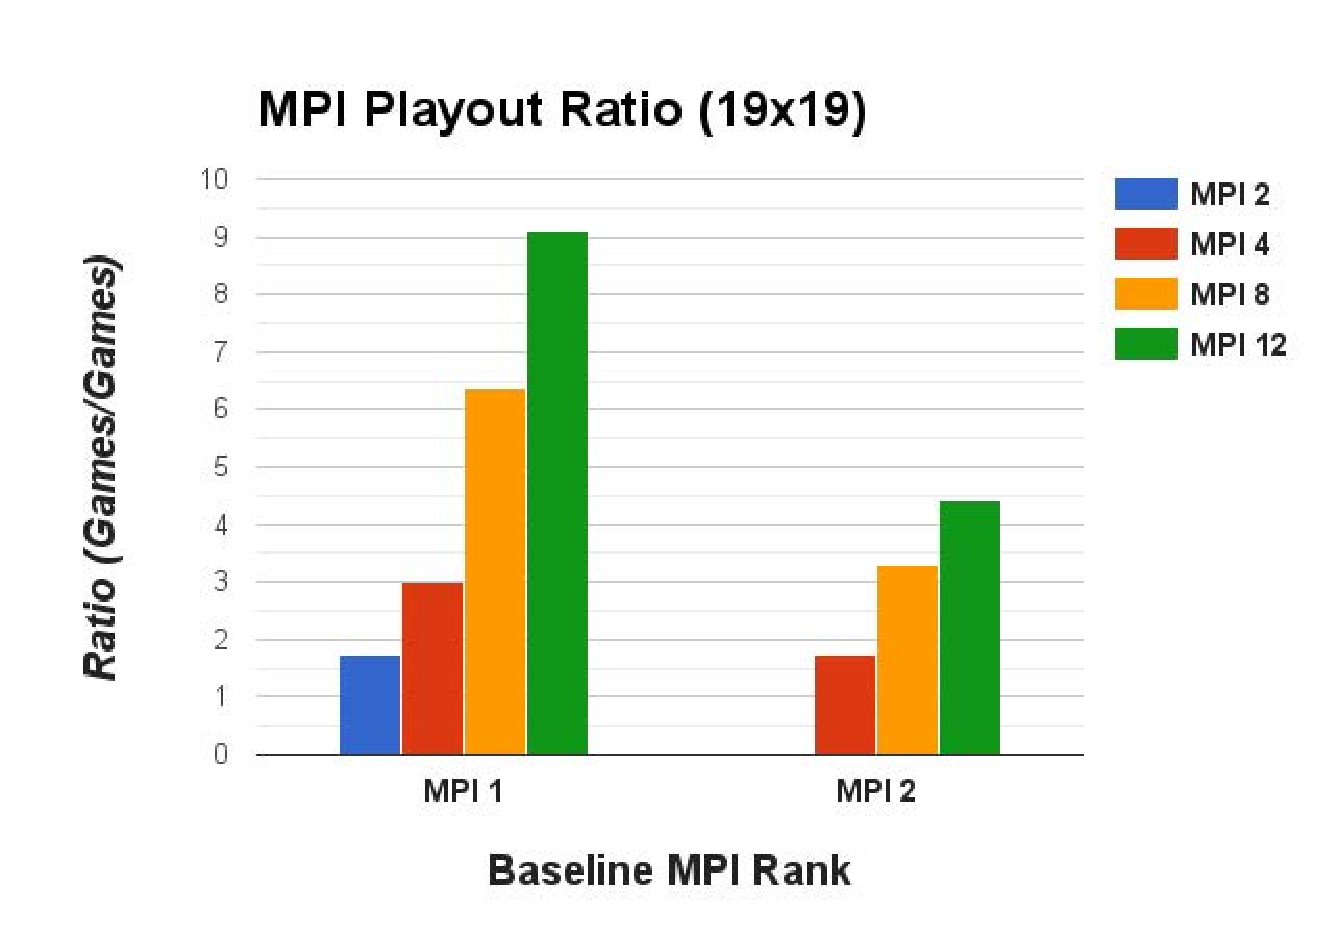
\includegraphics[width=0.45\textwidth]{MPI_playout_ratio_19x19.pdf}
\end{center}
\caption{The ratio of games explored for competing MPI configurations on a $19 \times 19$ board averaged over all 10 games.}
\label{fig:playoutmpifull}
\end{figure}


\begin{figure}
\begin{center}
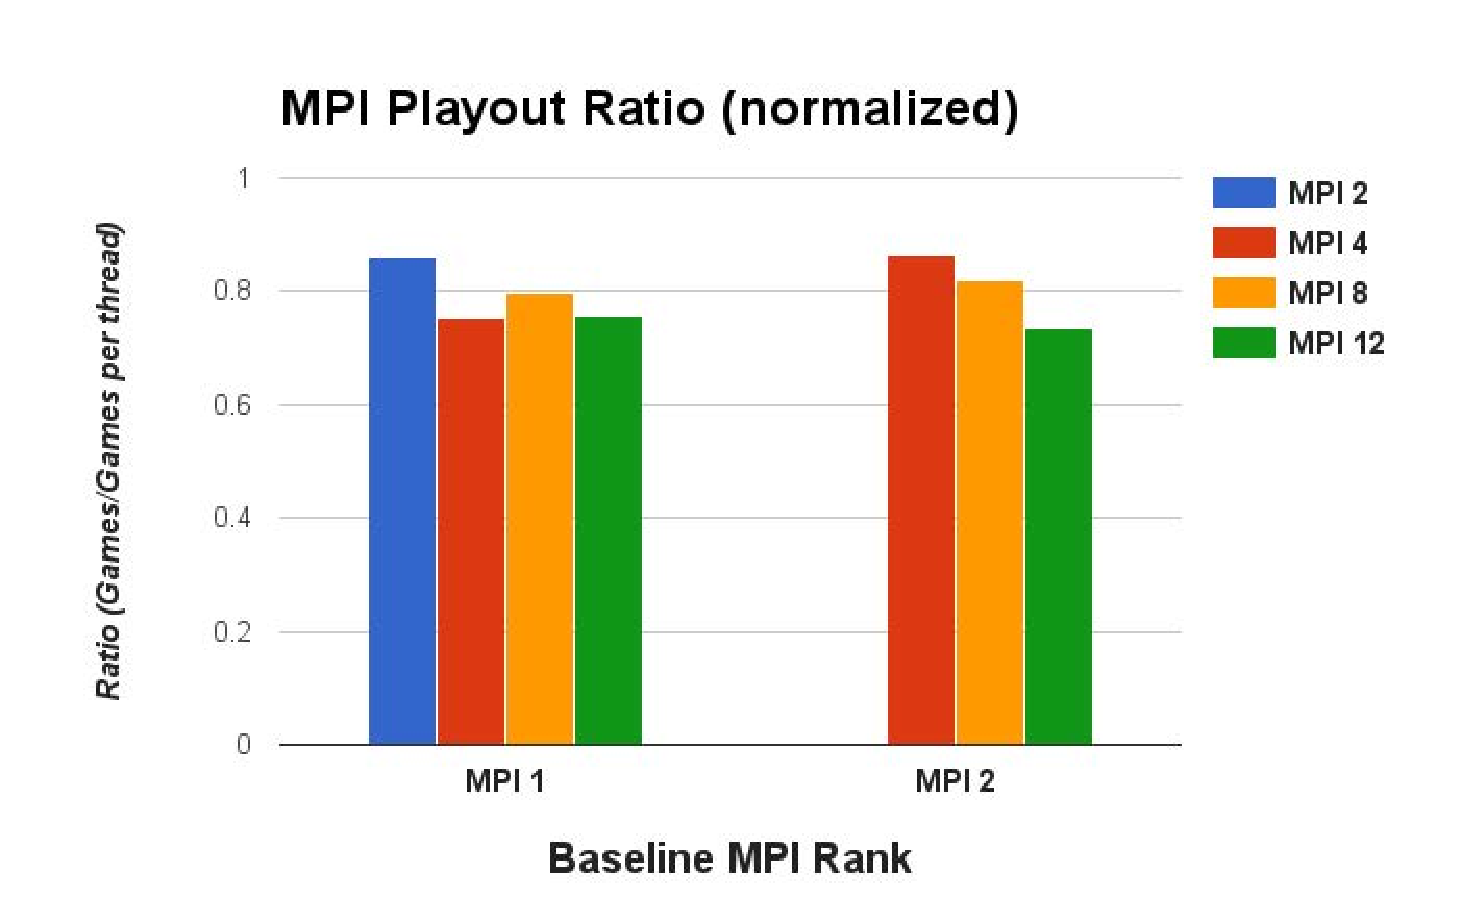
\includegraphics[width=0.45\textwidth]{MPI_playout_ratio_norm_19x19.pdf}
\end{center}
\caption{Normalized playout ratio for MPI on $19 \times 19$ boards. The normalization measures the thread factor advantage between competing MPI configurations.}
\label{fig:playoutmpifullnorm}
\end{figure}

Here we discuss the results generated from running simulations of games on $19\times 19$ boards in which we vary only the number of MPI ranks associated with each player. The player associated with white varied the number of ranks between 2, 4, 8 and 12 while the player associated with black varied the number of ranks between 1 and 2.  In all MPI games played on the large board, the player with the larger number of ranks was able to win 100\% of the time.  Figure~\ref{fig:playoutmpifull}, contains the ratio of playout results of these experiments.  From the graph it can be seen that for a given baseline MPI rank, increasing the MPI rank of the challenger causes the ratio between the number of playout games to increase.  Additionally, we see that as we increase the number of ranks associated with the baseline, the resulting ratio decreases.  To demonstrate the consistency of these changes, we have normalized the playout ratios by dividing by the ratio of the number of ranks associated with each player.  The resulting plot can be seen in Figure~\ref{fig:playoutmpifullnorm}.  We see that in general, this ratio remains relatively constant, demonstrating that our MPI parallel implementation scalable.

\section{Observations}

\subsection{Effects of Problem Size and Isoefficiency}

As one increases the number of processors one can explore additional games.  While these games will occur independently from one another, there is no guarantee of uniqueness.  It remains probabilistically possible that two explored games between different threads (or even on the same thread) result in identical play outs.  Due to vast number of moves generally possible within the game, this is a trivial issue.  However, this condition becomes important near the end of games, specifically whenever the number of possible combination of moves has decreased below the exploration threshold. 

As the exploration threshold is larger for multi-threaded executions, this threshold, at which all possible games from a given state are being explored, will occur sooner for multi-threaded expectations than for single threaded executions.  However, as the board is filling up, this point will eventually be reached by both players.  In such instances, both single and multi-threaded players have equal access to all possible game combinations, and any advantage gained through parallelization is lost in repetitive exploration.  Fortunately, on large boards, this point occurs late enough in the game that it is generally too late for the less parallel application to win.  However, in considering smaller boards, this point occurs early enough to allow the less parallel paler to occasionally win.  Thus for larger game boards, the parallel version will generally always win (100\% of the time) while in smaller boards, the less parallel version can occasionally win.  Such was clearly manifested in the outcomes of our games (noting that the less parallel version still never won a majority of the games).

%In a 9x9 grid, where the number of games is small or towards the end of the game where there are just a few possible games, increasing the number of processors does not result in better decisions, since one can explore the entire game space with less processors.

This is similar to the observation made by Gustafson which states that arbitrary large datasets can be efficiently parallelized. And has been shown experimentally in other studies when using Monte Carlo to play Go~\cite{DBLP:journals/corr/MirsoleimaniPVH14,SCAI11}.

\subsection{Branch Prediction Behavior}

Since the  Monte Carlo algorithm places stones randomly on the board and then checks if it can place the stone at that location, it has bad branch predicting behavior when the board is populated. To see that one must consider the case when we are playing around the middle of the game. Around half of the board is full and when we choose a random move the probability of the move being valid (not landing on top of another stone) is going to be 1/2. In this scenario, which arises at every iteration of the game the branch predictor fails each time. We have observed this by examining the runtime as well as running the Intel VTune analyzer~\cite{vtune} on the program.


\subsection{Cache Behavior}

As one increases the size of the board the program exhibits bad cache behavior. This is especially true when storing state at each position in the board and not just a bit signifying whether the position is occupied or not. When doing performance analysis on Pachi and other engines we observed that they have bad L1 cache behavior. We did do some low level optimizations (modifying how the structures are represented as well as the data size of the elements) to some of the engines and, while it did improve the L1 hit rate, we do believe that this form of cache behavior is inherit in tree search algorithms.





\section{Future Work}
\subsection{Monte Carlo Tree Search (MCTS)}
MCTS is a heuristic search algorithm which is used most notably in game playing. Unlike regular Monte Carlo, it concentrates on analyzing the most promising moves, basing the expansion of the search tree on random sampling of the search space. MTCS weighs the nodes of the game tree based on the outcome of playouts so that the better nodes are more likely to be chosen in future playouts. 

\begin{figure} [h]
\begin{center}
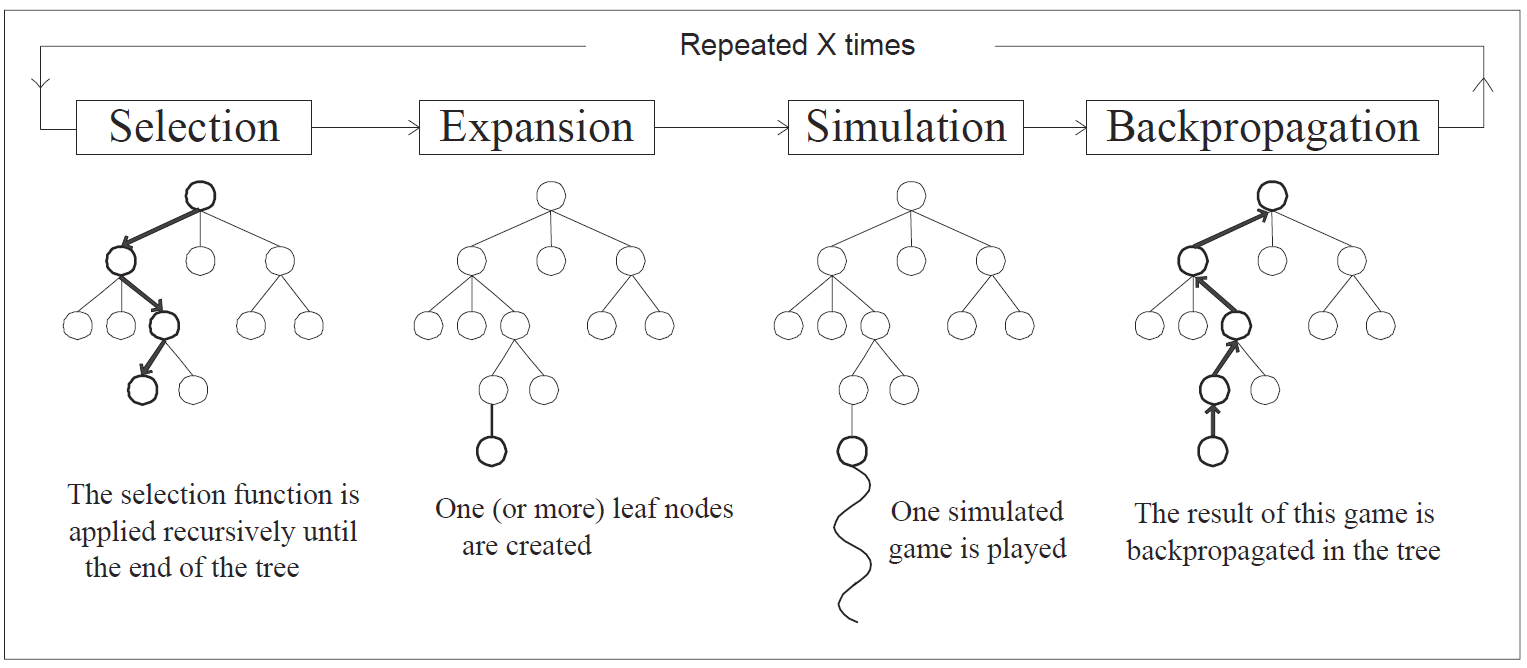
\includegraphics[scale=0.2]{MCTS.PNG}
\end{center}
\caption{Schematic describing the MCTS algorithm (Figure 1 in ~\cite{SCAI11}). The algorithm selects a favorable move, then explores the moves, performs a game simulation, and propagates the results back to root node.}
\label{MCTS}
\end{figure}

Each round of MCTS consists of four steps :
\begin{itemize}
\item Selection : starting from the Root, select successive child nodes down to a leaf node. 
\item Expansion : unless the leaf node ends the game, create more child nodes and select one of them
\item Simulation : play a random playout at the selected node
\item Backpropagation : update the information in the parent node based on the result of the playout
\end{itemize}

Figure ~\ref{MCTS} shows the four steps involved in MCTS. Such rounds are repeated as long as the time allotted for the move runs up. The node with the highest weight is chosen for the move. The information is recorded as part of the node's state so the next iteration would (a) not explore the same path, (b) would explore new paths. 


\begin{figure} [h]
\begin{center}
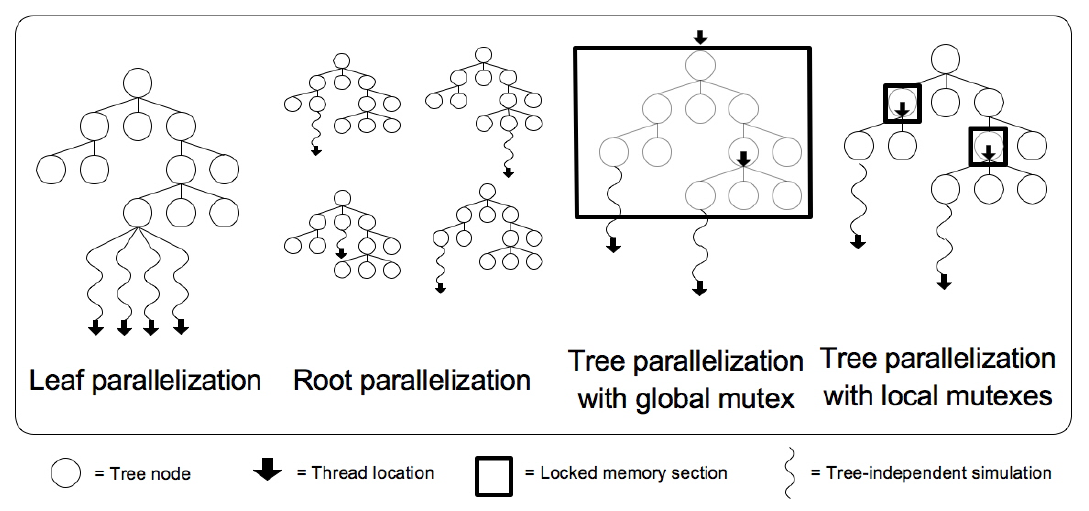
\includegraphics[scale=0.25]{PARMCTS.PNG}
\end{center}
\caption{The strategies used to parallelize the MCTS algorithm (Figure 2 in ~\cite{SCAI11}). Three different parallization strategies are shown each with their pros and cons.}
\label{PARMCTS}
\end{figure}

There are three different approaches to parallelization of MTCS as shown in Figure~\ref{PARMCTS} depending on which step of the Monte Carlo Tree Search is parallelized. The choice of what to parallelized results in different implementation inefficiencies and therefore different performance characteristics. Other studies have examined these in more detail~\cite{SCAI11,gpugo}, but we summarize the methods.

\textbf{Leaf Parallelization}

In leaf parallelization, only one thread traverses the tree and adds one or more nodes to the tree. Starting from the leaf node, independent simulated games are run in parallel on each available thread. When all the games finish, the result of all these games is propagated backwards by a single thread.

\textbf{Root Parallelization}

Root Parallelization works by growing the MCTS tree growing in parallel with one thread assigned a tree. Similar to leaf parallelization, the threads do not communicate with each other during game simulation. When the available time has passed or the play-outs are complete, all the root children of separate MCTS trees are merged and results are added. The best move is selected based on the total.

\textbf{Tree Parallelization}

Finally in tree parallelization, a common tree is shared and several simultaneous games are played. Each thread can modify the information contained in the tree and therefore communication between threads is required. Performing optimal sharing is difficult to implement compared to other methods of parallelization. In practice the sharing is implemented using local or global locks --- making this method more inefficient.

In practice the leaf parallelization is the easiest to implement, the root parallelization is the most efficient, and the tree parallelization is complex and inefficient.

\subsection{Algorithm Applications}

The MCTS algorithm is interesting since it has applications outside game AI. It has been used 
to solve satisfiability problems~\cite{mcstsat}, planning problems~\cite{mcstplan}, and more~\cite{mcstsurv}. One interesting application that we found is using MCTS to efficiently
represent polynomial equations for compilation. Some compilers already employ Horner's form~\cite{horner} or Estrin's scheme~\cite{estrin}, but the factorized polynomial generated by these methods have wide performance characteristics depending on which variable is chosen during factorization. In FORM~\cite{form} and Hepgame~\cite{hepgame} they use MCTS to optimize the polynomials giving them huge runtime benefits\footnote{The polynomials arise when tyring to solve equations using Feynman diagrams. They also arise due to Sylvester's identity~\cite{sylv} which states that two polynomials have simultaneous solutions if the Sylvester determinant is non-zero~\cite{polyeval}. }

\subsection{Additional Evaluations}


Future work would concentrate on performing analysis of the space between MPI and OpenMP on the full $19 \times 19$ board. While we did show how the behavior of the algorithm changes on the full board, due to time and resource constraints the space of MPI and OpenMP was not explored in detail as we had wanted. Comparing our parallel implementation against a tree pruning method would also be interesting, since while the tree pruning methods avoid work we can exploit the fact that we can perform more work in the allotted time. We can therefore be more eager in our exploration step. Finally, pitting our engine against human players would allow us to tell how well a Monte Carlo implementation fairs against a human.

\begin{thebibliography}{9}
\bibitem{pachi} Baudiš, Petr, and Jean-loup Gailly. "Pachi: State of the art open source Go program." Advances in Computer Games. Springer Berlin Heidelberg, 2012. 24-38.
\bibitem{gohard} Levinovitz, Alan. "The Mystery of Go, the Ancient Game That Computers Still Can’t Win." Wired.com. Conde Nast Digital, 12 May 2014. Web. 12 May 2015.
\bibitem{DBLP:journals/corr/MirsoleimaniPVH14} Ali M. et al Performance analysis of a 240 thread tournament level MCTS Go program on the Intel Xeon Phi 2014
\bibitem{SCAI11} Rocki, Kamil, and Reiji Suda. "Parallel Monte Carlo Tree Search on GPU." SCAI. 2011.
\bibitem{vtune} Sridharan, K. "VTune: Intel’s Visual Tuning Environment." Proceedings of USENIX-NT’97 11 (1997).
\bibitem{branch} "Branching Factor." Wikipedia. Wikimedia Foundation, n.d. Web. 12 May 2015.
\bibitem{abvs} Jakl, Tomáš, and Tomáš Jakl. "Arimaa challenge–Comparission study of MCTS versus alpha-beta methods." Memory 37 (2011): 37-5.
\bibitem{mathgo} "Go and Mathematics." Wikipedia. Wikimedia Foundation, n.d. Web. 12 May 2015.
\bibitem{deepblue} "Deep Blue (chess Computer)." Wikipedia. Wikimedia Foundation, n.d. Web. 12 May 2015.
\bibitem{exptime} Robson, John Michael. "The Complexity of Go." IFIP Congress. 1983.
\bibitem{exptime2} Lichtenstein, David, and Michael Sipser. "Go is polynomial-space hard." Journal of the ACM (JACM) 27.2 (1980): 393-401.
\bibitem{mcstsat} Okamoto, Yoshio, and Takeaki Uno. "A polynomial-time-delay and polynomial-space algorithm for enumeration problems in multi-criteria optimization." European Journal of Operational Research 210.1 (2011): 48-56.
\bibitem{mcstplan} Lee, Taekhee, and Young J. Kim. "GPU-based Motion Planning under Uncertainties using POMDP." Robotics and Automation (ICRA), 2013 IEEE International Conference on. IEEE, 2013.
\bibitem{mcstsurv} Browne, Cameron B., et al. "A survey of monte carlo tree search methods." Computational Intelligence and AI in Games, IEEE Transactions on 4.1 (2012): 1-43.
\bibitem{horner} Weisstein, Eric W. "Horner's Method." From MathWorld--A Wolfram Web Resource. http://mathworld.wolfram.com/HornersMethod.html
\bibitem{estrin} G. Estrin, Organization of computer systems - The fixed plus variable structure computer, in Proc. Western Joint Comput. Conf., May 1960, pp. 33-40.
\bibitem{form} Kuipers, J., T. Ueda, and J. A. M. Vermaseren. "Code optimization in FORM." Computer Physics Communications (2014).
\bibitem{hepgame} Ruijl, Ben, et al. "HEPGAME and the Simplification of Expressions." arXiv preprint arXiv:1405.6369 (2014).
\bibitem{sylv} Weisstein, Eric W. "Sylvester's Determinant Identity." From MathWorld--A Wolfram Web Resource. http://mathworld.wolfram.com/SylvestersDeterminantIdentity.html
\bibitem{polyeval} Leiserson, Charles E., et al. "Efficient evaluation of large polynomials." Mathematical Software–ICMS 2010. Springer Berlin Heidelberg, 2010. 342-353.
\bibitem{gpugo} Barriga, Nicolas A., Marius Stanescu, and Michael Buro. "Parallel UCT search on GPUs." Computational Intelligence and Games (CIG), 2014 IEEE Conference on. IEEE, 2014.
\end{thebibliography}
\end{document}